% Options for packages loaded elsewhere
\PassOptionsToPackage{unicode}{hyperref}
\PassOptionsToPackage{hyphens}{url}
%
\documentclass[
]{article}
\usepackage{amsmath,amssymb}
\usepackage{iftex}
\ifPDFTeX
  \usepackage[T1]{fontenc}
  \usepackage[utf8]{inputenc}
  \usepackage{textcomp} % provide euro and other symbols
\else % if luatex or xetex
  \usepackage{unicode-math} % this also loads fontspec
  \defaultfontfeatures{Scale=MatchLowercase}
  \defaultfontfeatures[\rmfamily]{Ligatures=TeX,Scale=1}
\fi
\usepackage{lmodern}
\ifPDFTeX\else
  % xetex/luatex font selection
\fi
% Use upquote if available, for straight quotes in verbatim environments
\IfFileExists{upquote.sty}{\usepackage{upquote}}{}
\IfFileExists{microtype.sty}{% use microtype if available
  \usepackage[]{microtype}
  \UseMicrotypeSet[protrusion]{basicmath} % disable protrusion for tt fonts
}{}
\makeatletter
\@ifundefined{KOMAClassName}{% if non-KOMA class
  \IfFileExists{parskip.sty}{%
    \usepackage{parskip}
  }{% else
    \setlength{\parindent}{0pt}
    \setlength{\parskip}{6pt plus 2pt minus 1pt}}
}{% if KOMA class
  \KOMAoptions{parskip=half}}
\makeatother
\usepackage{xcolor}
\usepackage[margin=1in]{geometry}
\usepackage{color}
\usepackage{fancyvrb}
\newcommand{\VerbBar}{|}
\newcommand{\VERB}{\Verb[commandchars=\\\{\}]}
\DefineVerbatimEnvironment{Highlighting}{Verbatim}{commandchars=\\\{\}}
% Add ',fontsize=\small' for more characters per line
\usepackage{framed}
\definecolor{shadecolor}{RGB}{248,248,248}
\newenvironment{Shaded}{\begin{snugshade}}{\end{snugshade}}
\newcommand{\AlertTok}[1]{\textcolor[rgb]{0.94,0.16,0.16}{#1}}
\newcommand{\AnnotationTok}[1]{\textcolor[rgb]{0.56,0.35,0.01}{\textbf{\textit{#1}}}}
\newcommand{\AttributeTok}[1]{\textcolor[rgb]{0.13,0.29,0.53}{#1}}
\newcommand{\BaseNTok}[1]{\textcolor[rgb]{0.00,0.00,0.81}{#1}}
\newcommand{\BuiltInTok}[1]{#1}
\newcommand{\CharTok}[1]{\textcolor[rgb]{0.31,0.60,0.02}{#1}}
\newcommand{\CommentTok}[1]{\textcolor[rgb]{0.56,0.35,0.01}{\textit{#1}}}
\newcommand{\CommentVarTok}[1]{\textcolor[rgb]{0.56,0.35,0.01}{\textbf{\textit{#1}}}}
\newcommand{\ConstantTok}[1]{\textcolor[rgb]{0.56,0.35,0.01}{#1}}
\newcommand{\ControlFlowTok}[1]{\textcolor[rgb]{0.13,0.29,0.53}{\textbf{#1}}}
\newcommand{\DataTypeTok}[1]{\textcolor[rgb]{0.13,0.29,0.53}{#1}}
\newcommand{\DecValTok}[1]{\textcolor[rgb]{0.00,0.00,0.81}{#1}}
\newcommand{\DocumentationTok}[1]{\textcolor[rgb]{0.56,0.35,0.01}{\textbf{\textit{#1}}}}
\newcommand{\ErrorTok}[1]{\textcolor[rgb]{0.64,0.00,0.00}{\textbf{#1}}}
\newcommand{\ExtensionTok}[1]{#1}
\newcommand{\FloatTok}[1]{\textcolor[rgb]{0.00,0.00,0.81}{#1}}
\newcommand{\FunctionTok}[1]{\textcolor[rgb]{0.13,0.29,0.53}{\textbf{#1}}}
\newcommand{\ImportTok}[1]{#1}
\newcommand{\InformationTok}[1]{\textcolor[rgb]{0.56,0.35,0.01}{\textbf{\textit{#1}}}}
\newcommand{\KeywordTok}[1]{\textcolor[rgb]{0.13,0.29,0.53}{\textbf{#1}}}
\newcommand{\NormalTok}[1]{#1}
\newcommand{\OperatorTok}[1]{\textcolor[rgb]{0.81,0.36,0.00}{\textbf{#1}}}
\newcommand{\OtherTok}[1]{\textcolor[rgb]{0.56,0.35,0.01}{#1}}
\newcommand{\PreprocessorTok}[1]{\textcolor[rgb]{0.56,0.35,0.01}{\textit{#1}}}
\newcommand{\RegionMarkerTok}[1]{#1}
\newcommand{\SpecialCharTok}[1]{\textcolor[rgb]{0.81,0.36,0.00}{\textbf{#1}}}
\newcommand{\SpecialStringTok}[1]{\textcolor[rgb]{0.31,0.60,0.02}{#1}}
\newcommand{\StringTok}[1]{\textcolor[rgb]{0.31,0.60,0.02}{#1}}
\newcommand{\VariableTok}[1]{\textcolor[rgb]{0.00,0.00,0.00}{#1}}
\newcommand{\VerbatimStringTok}[1]{\textcolor[rgb]{0.31,0.60,0.02}{#1}}
\newcommand{\WarningTok}[1]{\textcolor[rgb]{0.56,0.35,0.01}{\textbf{\textit{#1}}}}
\usepackage{graphicx}
\makeatletter
\def\maxwidth{\ifdim\Gin@nat@width>\linewidth\linewidth\else\Gin@nat@width\fi}
\def\maxheight{\ifdim\Gin@nat@height>\textheight\textheight\else\Gin@nat@height\fi}
\makeatother
% Scale images if necessary, so that they will not overflow the page
% margins by default, and it is still possible to overwrite the defaults
% using explicit options in \includegraphics[width, height, ...]{}
\setkeys{Gin}{width=\maxwidth,height=\maxheight,keepaspectratio}
% Set default figure placement to htbp
\makeatletter
\def\fps@figure{htbp}
\makeatother
\setlength{\emergencystretch}{3em} % prevent overfull lines
\providecommand{\tightlist}{%
  \setlength{\itemsep}{0pt}\setlength{\parskip}{0pt}}
\setcounter{secnumdepth}{-\maxdimen} % remove section numbering
\ifLuaTeX
  \usepackage{selnolig}  % disable illegal ligatures
\fi
\usepackage{bookmark}
\IfFileExists{xurl.sty}{\usepackage{xurl}}{} % add URL line breaks if available
\urlstyle{same}
\hypersetup{
  pdftitle={Entrega2\_Proyecto1},
  pdfauthor={Gustavo Cruz; Pedro Guzman},
  hidelinks,
  pdfcreator={LaTeX via pandoc}}

\title{Entrega2\_Proyecto1}
\author{Gustavo Cruz; Pedro Guzman}
\date{2025-02-12}

\begin{document}
\maketitle

Repositorio: \url{https://github.com/G2309/MD_Proyecto2.git}

\begin{Shaded}
\begin{Highlighting}[]
\NormalTok{movies }\OtherTok{\textless{}{-}} \FunctionTok{read.csv}\NormalTok{(}\StringTok{\textquotesingle{}movies.csv\textquotesingle{}}\NormalTok{, }\AttributeTok{stringsAsFactors =} \ConstantTok{FALSE}\NormalTok{)}
\end{Highlighting}
\end{Shaded}

\subsection{Determinación de la cantidad de
grupos}\label{determinaciuxf3n-de-la-cantidad-de-grupos}

\begin{Shaded}
\begin{Highlighting}[]
\FunctionTok{library}\NormalTok{(tidyverse)}
\end{Highlighting}
\end{Shaded}

\begin{verbatim}
## -- Attaching core tidyverse packages ------------------------ tidyverse 2.0.0 --
## v dplyr     1.1.4     v readr     2.1.5
## v forcats   1.0.0     v stringr   1.5.1
## v ggplot2   3.5.1     v tibble    3.2.1
## v lubridate 1.9.4     v tidyr     1.3.1
## v purrr     1.0.4     
## -- Conflicts ------------------------------------------ tidyverse_conflicts() --
## x dplyr::filter() masks stats::filter()
## x dplyr::lag()    masks stats::lag()
## i Use the conflicted package (<http://conflicted.r-lib.org/>) to force all conflicts to become errors
\end{verbatim}

\begin{Shaded}
\begin{Highlighting}[]
\FunctionTok{library}\NormalTok{(cluster)}
\FunctionTok{library}\NormalTok{(factoextra)}
\end{Highlighting}
\end{Shaded}

\begin{verbatim}
## Welcome! Want to learn more? See two factoextra-related books at https://goo.gl/ve3WBa
\end{verbatim}

\begin{Shaded}
\begin{Highlighting}[]
\CommentTok{\# Función para remover outliers usando IQR}
\NormalTok{remove\_outliers }\OtherTok{\textless{}{-}} \ControlFlowTok{function}\NormalTok{(x) \{}
\NormalTok{  qnt }\OtherTok{\textless{}{-}} \FunctionTok{quantile}\NormalTok{(x, }\AttributeTok{probs=}\FunctionTok{c}\NormalTok{(.}\DecValTok{25}\NormalTok{, .}\DecValTok{75}\NormalTok{), }\AttributeTok{na.rm=}\ConstantTok{TRUE}\NormalTok{)}
\NormalTok{  H }\OtherTok{\textless{}{-}} \FloatTok{1.5} \SpecialCharTok{*} \FunctionTok{IQR}\NormalTok{(x, }\AttributeTok{na.rm=}\ConstantTok{TRUE}\NormalTok{)}
\NormalTok{  x[x }\SpecialCharTok{\textless{}}\NormalTok{ (qnt[}\DecValTok{1}\NormalTok{] }\SpecialCharTok{{-}}\NormalTok{ H)] }\OtherTok{\textless{}{-}} \ConstantTok{NA}
\NormalTok{  x[x }\SpecialCharTok{\textgreater{}}\NormalTok{ (qnt[}\DecValTok{2}\NormalTok{] }\SpecialCharTok{+}\NormalTok{ H)] }\OtherTok{\textless{}{-}} \ConstantTok{NA}
  \FunctionTok{return}\NormalTok{(x)}
\NormalTok{\}}

\NormalTok{movies\_clean }\OtherTok{\textless{}{-}}\NormalTok{ movies }\SpecialCharTok{\%\textgreater{}\%}
  \FunctionTok{select}\NormalTok{(popularity, budget, revenue, runtime, }
\NormalTok{         genresAmount, productionCoAmount, }
\NormalTok{         productionCountriesAmount, voteCount, }
\NormalTok{         voteAvg, actorsAmount, }
\NormalTok{         castWomenAmount, castMenAmount) }\SpecialCharTok{\%\textgreater{}\%}
  \FunctionTok{mutate}\NormalTok{(}\FunctionTok{across}\NormalTok{(}\FunctionTok{everything}\NormalTok{(), as.numeric)) }\SpecialCharTok{\%\textgreater{}\%}
  \CommentTok{\# Remover outliers}
  \FunctionTok{mutate}\NormalTok{(}\FunctionTok{across}\NormalTok{(}\FunctionTok{everything}\NormalTok{(), remove\_outliers)) }\SpecialCharTok{\%\textgreater{}\%}
  \CommentTok{\# Eliminar filas con NA}
  \FunctionTok{na.omit}\NormalTok{()}

\NormalTok{movies\_scaled }\OtherTok{\textless{}{-}} \FunctionTok{scale}\NormalTok{(movies\_clean)}

\FunctionTok{set.seed}\NormalTok{(}\DecValTok{531}\NormalTok{) }\CommentTok{\# Seed para reproducibilidad}
\NormalTok{wss }\OtherTok{\textless{}{-}} \FunctionTok{numeric}\NormalTok{(}\DecValTok{12}\NormalTok{)  }
\ControlFlowTok{for}\NormalTok{ (k }\ControlFlowTok{in} \DecValTok{1}\SpecialCharTok{:}\DecValTok{12}\NormalTok{) \{}
\NormalTok{  km }\OtherTok{\textless{}{-}} \FunctionTok{kmeans}\NormalTok{(movies\_scaled, }
               \AttributeTok{centers =}\NormalTok{ k, }
               \AttributeTok{nstart =} \DecValTok{50}\NormalTok{,  }
               \AttributeTok{iter.max =} \DecValTok{50}\NormalTok{)  }
\NormalTok{  wss[k] }\OtherTok{\textless{}{-}}\NormalTok{ km}\SpecialCharTok{$}\NormalTok{tot.withinss}
\NormalTok{\}}

\NormalTok{p }\OtherTok{\textless{}{-}} \FunctionTok{fviz\_nbclust}\NormalTok{(movies\_scaled, }
\NormalTok{             kmeans, }
             \AttributeTok{method =} \StringTok{"wss"}\NormalTok{,}
             \AttributeTok{k.max =} \DecValTok{12}\NormalTok{,  }
             \AttributeTok{nstart =} \DecValTok{50}\NormalTok{,  }
             \AttributeTok{iter.max =} \DecValTok{50}\NormalTok{) }\SpecialCharTok{+}  
  \FunctionTok{labs}\NormalTok{(}\AttributeTok{title =} \StringTok{"Método del Codo para Determinar k Óptimo"}\NormalTok{,}
       \AttributeTok{x =} \StringTok{"Número de Clusters (k)"}\NormalTok{,}
       \AttributeTok{y =} \StringTok{"Suma total de cuadrados dentro de clusters"}\NormalTok{) }\SpecialCharTok{+}
  \FunctionTok{theme\_minimal}\NormalTok{()}

\FunctionTok{print}\NormalTok{(p)}
\end{Highlighting}
\end{Shaded}

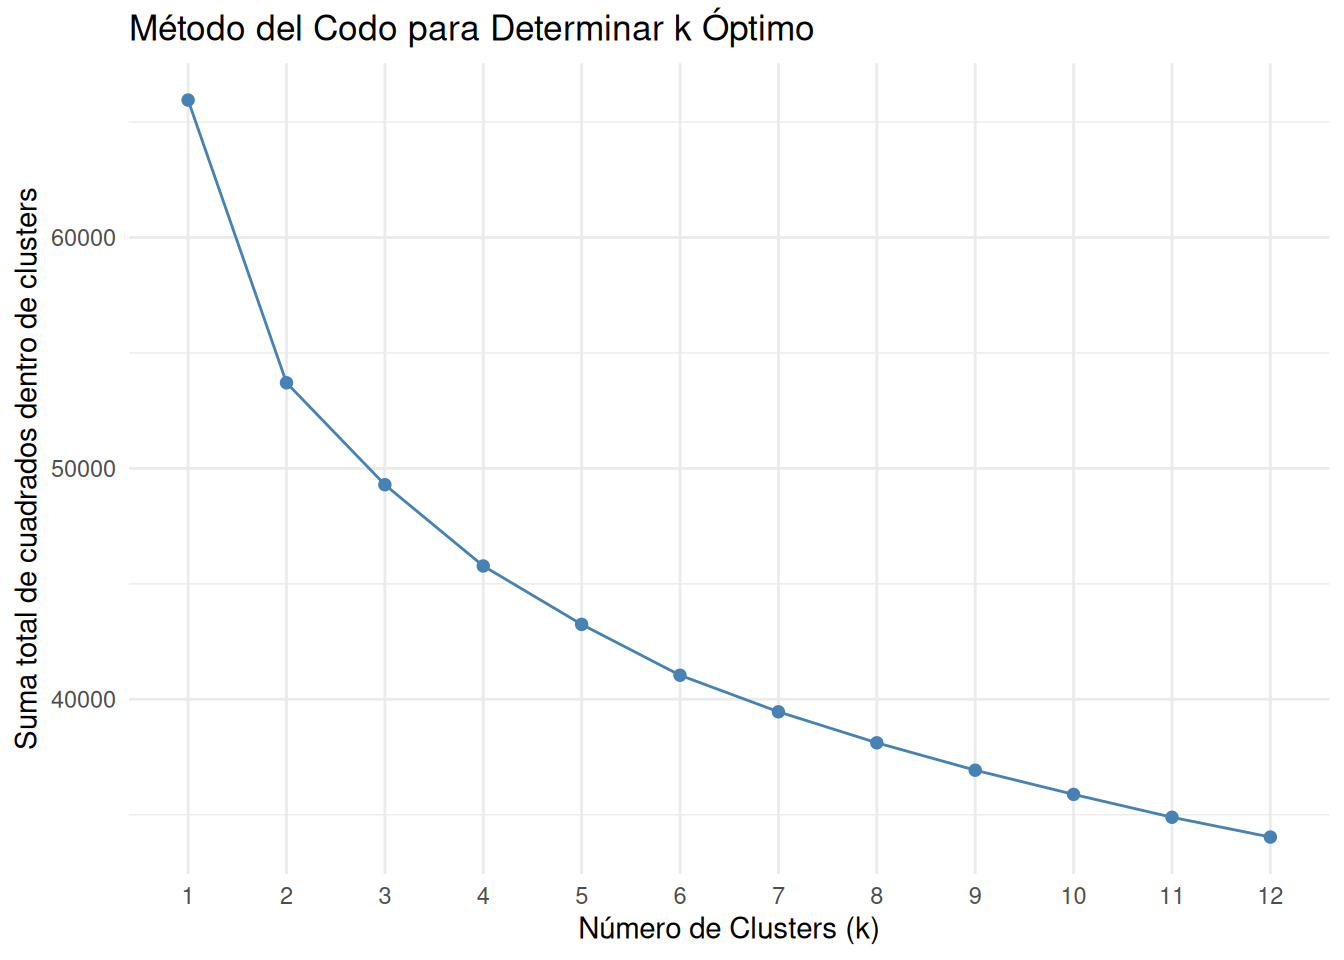
\includegraphics{Reporte_Entrega2_Proyecto1_files/figure-latex/unnamed-chunk-2-1.pdf}

\begin{Shaded}
\begin{Highlighting}[]
\NormalTok{wss\_diff }\OtherTok{\textless{}{-}} \FunctionTok{diff}\NormalTok{(wss) }\SpecialCharTok{/}\NormalTok{ wss[}\SpecialCharTok{{-}}\FunctionTok{length}\NormalTok{(wss)] }\SpecialCharTok{*} \DecValTok{100}
\FunctionTok{print}\NormalTok{(}\StringTok{"}\SpecialCharTok{\textbackslash{}n}\StringTok{Reducción porcentual en WSS para cada k adicional:"}\NormalTok{)}
\end{Highlighting}
\end{Shaded}

\begin{verbatim}
## [1] "\nReducción porcentual en WSS para cada k adicional:"
\end{verbatim}

\begin{Shaded}
\begin{Highlighting}[]
\ControlFlowTok{for}\NormalTok{(i }\ControlFlowTok{in} \DecValTok{1}\SpecialCharTok{:}\FunctionTok{length}\NormalTok{(wss\_diff)) \{}
  \FunctionTok{cat}\NormalTok{(}\FunctionTok{sprintf}\NormalTok{(}\StringTok{"De \%d a \%d clusters: \%.2f\%\% de reducción}\SpecialCharTok{\textbackslash{}n}\StringTok{"}\NormalTok{, }
\NormalTok{              i, i}\SpecialCharTok{+}\DecValTok{1}\NormalTok{, }\FunctionTok{abs}\NormalTok{(wss\_diff[i])))}
\NormalTok{\}}
\end{Highlighting}
\end{Shaded}

\begin{verbatim}
## De 1 a 2 clusters: 18.56% de reducción
## De 2 a 3 clusters: 8.22% de reducción
## De 3 a 4 clusters: 7.14% de reducción
## De 4 a 5 clusters: 5.53% de reducción
## De 5 a 6 clusters: 5.09% de reducción
## De 6 a 7 clusters: 3.86% de reducción
## De 7 a 8 clusters: 3.40% de reducción
## De 8 a 9 clusters: 3.12% de reducción
## De 9 a 10 clusters: 2.84% de reducción
## De 10 a 11 clusters: 2.76% de reducción
## De 11 a 12 clusters: 2.46% de reducción
\end{verbatim}

\subsection{Agrupamiento}\label{agrupamiento}

\begin{Shaded}
\begin{Highlighting}[]
\CommentTok{\# Para el ejercicio 2 de clustering estare utilizando la seed 531}
\NormalTok{movies\_clean }\OtherTok{\textless{}{-}}\NormalTok{ movies }\SpecialCharTok{\%\textgreater{}\%}
  \FunctionTok{select}\NormalTok{(popularity, budget, revenue, runtime, }
\NormalTok{         genresAmount, productionCoAmount, }
\NormalTok{         productionCountriesAmount, voteCount, }
\NormalTok{         voteAvg, actorsAmount, }
\NormalTok{         castWomenAmount, castMenAmount) }\SpecialCharTok{\%\textgreater{}\%}
  \FunctionTok{mutate}\NormalTok{(}\FunctionTok{across}\NormalTok{(}\FunctionTok{everything}\NormalTok{(), as.numeric)) }\SpecialCharTok{\%\textgreater{}\%}
  \FunctionTok{mutate}\NormalTok{(}\FunctionTok{across}\NormalTok{(}\FunctionTok{everything}\NormalTok{(), remove\_outliers)) }\SpecialCharTok{\%\textgreater{}\%}
  \FunctionTok{na.omit}\NormalTok{()}

\NormalTok{movies\_scaled }\OtherTok{\textless{}{-}} \FunctionTok{scale}\NormalTok{(movies\_clean)}

\FunctionTok{set.seed}\NormalTok{(}\DecValTok{531}\NormalTok{)}
\NormalTok{kmeans\_result }\OtherTok{\textless{}{-}} \FunctionTok{kmeans}\NormalTok{(movies\_scaled, }
                       \AttributeTok{centers =} \DecValTok{4}\NormalTok{, }
                       \AttributeTok{nstart =} \DecValTok{50}\NormalTok{,}
                       \AttributeTok{iter.max =} \DecValTok{50}\NormalTok{)}

\FunctionTok{set.seed}\NormalTok{(}\DecValTok{531}\NormalTok{)}
\NormalTok{sample\_size }\OtherTok{\textless{}{-}} \FunctionTok{min}\NormalTok{(}\DecValTok{1000}\NormalTok{, }\FunctionTok{nrow}\NormalTok{(movies\_scaled))}
\NormalTok{sample\_indices }\OtherTok{\textless{}{-}} \FunctionTok{sample}\NormalTok{(}\DecValTok{1}\SpecialCharTok{:}\FunctionTok{nrow}\NormalTok{(movies\_scaled), sample\_size)}
\NormalTok{movies\_sample }\OtherTok{\textless{}{-}}\NormalTok{ movies\_scaled[sample\_indices, ]}

\NormalTok{dist\_matrix }\OtherTok{\textless{}{-}} \FunctionTok{dist}\NormalTok{(movies\_sample, }\AttributeTok{method =} \StringTok{"euclidean"}\NormalTok{)}
\NormalTok{hclust\_result }\OtherTok{\textless{}{-}} \FunctionTok{hclust}\NormalTok{(dist\_matrix, }\AttributeTok{method =} \StringTok{"ward.D2"}\NormalTok{)}
\NormalTok{hclust\_clusters }\OtherTok{\textless{}{-}} \FunctionTok{cutree}\NormalTok{(hclust\_result, }\AttributeTok{k =} \DecValTok{4}\NormalTok{)}

\NormalTok{silhouette\_kmeans }\OtherTok{\textless{}{-}} \FunctionTok{silhouette}\NormalTok{(kmeans\_result}\SpecialCharTok{$}\NormalTok{cluster, }
                               \FunctionTok{dist}\NormalTok{(movies\_scaled))}
\NormalTok{sil\_score\_kmeans }\OtherTok{\textless{}{-}} \FunctionTok{mean}\NormalTok{(silhouette\_kmeans[,}\DecValTok{3}\NormalTok{])}

\NormalTok{silhouette\_hclust }\OtherTok{\textless{}{-}} \FunctionTok{silhouette}\NormalTok{(hclust\_clusters, dist\_matrix)}
\NormalTok{sil\_score\_hclust }\OtherTok{\textless{}{-}} \FunctionTok{mean}\NormalTok{(silhouette\_hclust[,}\DecValTok{3}\NormalTok{])}

\FunctionTok{cat}\NormalTok{(}\StringTok{"}\SpecialCharTok{\textbackslash{}n}\StringTok{Comparación de Algoritmos de Clustering:}\SpecialCharTok{\textbackslash{}n}\StringTok{"}\NormalTok{)}
\end{Highlighting}
\end{Shaded}

\begin{verbatim}
## 
## Comparación de Algoritmos de Clustering:
\end{verbatim}

\begin{Shaded}
\begin{Highlighting}[]
\FunctionTok{cat}\NormalTok{(}\StringTok{"}\SpecialCharTok{\textbackslash{}n}\StringTok{K{-}means:"}\NormalTok{)}
\end{Highlighting}
\end{Shaded}

\begin{verbatim}
## 
## K-means:
\end{verbatim}

\begin{Shaded}
\begin{Highlighting}[]
\FunctionTok{cat}\NormalTok{(}\StringTok{"}\SpecialCharTok{\textbackslash{}n}\StringTok{{-} Número de observaciones por cluster:}\SpecialCharTok{\textbackslash{}n}\StringTok{"}\NormalTok{)}
\end{Highlighting}
\end{Shaded}

\begin{verbatim}
## 
## - Número de observaciones por cluster:
\end{verbatim}

\begin{Shaded}
\begin{Highlighting}[]
\FunctionTok{print}\NormalTok{(}\FunctionTok{table}\NormalTok{(kmeans\_result}\SpecialCharTok{$}\NormalTok{cluster))}
\end{Highlighting}
\end{Shaded}

\begin{verbatim}
## 
##    1    2    3    4 
## 1315  796  873 2513
\end{verbatim}

\begin{Shaded}
\begin{Highlighting}[]
\FunctionTok{cat}\NormalTok{(}\StringTok{"}\SpecialCharTok{\textbackslash{}n}\StringTok{{-} Coeficiente de silueta promedio:"}\NormalTok{, }\FunctionTok{round}\NormalTok{(sil\_score\_kmeans, }\DecValTok{3}\NormalTok{))}
\end{Highlighting}
\end{Shaded}

\begin{verbatim}
## 
## - Coeficiente de silueta promedio: 0.145
\end{verbatim}

\begin{Shaded}
\begin{Highlighting}[]
\FunctionTok{cat}\NormalTok{(}\StringTok{"}\SpecialCharTok{\textbackslash{}n\textbackslash{}n}\StringTok{Clustering Jerárquico (muestra de"}\NormalTok{, sample\_size, }\StringTok{"observaciones):"}\NormalTok{)}
\end{Highlighting}
\end{Shaded}

\begin{verbatim}
## 
## 
## Clustering Jerárquico (muestra de 1000 observaciones):
\end{verbatim}

\begin{Shaded}
\begin{Highlighting}[]
\FunctionTok{cat}\NormalTok{(}\StringTok{"}\SpecialCharTok{\textbackslash{}n}\StringTok{{-} Número de observaciones por cluster:}\SpecialCharTok{\textbackslash{}n}\StringTok{"}\NormalTok{)}
\end{Highlighting}
\end{Shaded}

\begin{verbatim}
## 
## - Número de observaciones por cluster:
\end{verbatim}

\begin{Shaded}
\begin{Highlighting}[]
\FunctionTok{print}\NormalTok{(}\FunctionTok{table}\NormalTok{(hclust\_clusters))}
\end{Highlighting}
\end{Shaded}

\begin{verbatim}
## hclust_clusters
##   1   2   3   4 
## 572 114 116 198
\end{verbatim}

\begin{Shaded}
\begin{Highlighting}[]
\FunctionTok{cat}\NormalTok{(}\StringTok{"}\SpecialCharTok{\textbackslash{}n}\StringTok{{-} Coeficiente de silueta promedio:"}\NormalTok{, }\FunctionTok{round}\NormalTok{(sil\_score\_hclust, }\DecValTok{3}\NormalTok{))}
\end{Highlighting}
\end{Shaded}

\begin{verbatim}
## 
## - Coeficiente de silueta promedio: 0.105
\end{verbatim}

\begin{Shaded}
\begin{Highlighting}[]
\NormalTok{pca\_result }\OtherTok{\textless{}{-}} \FunctionTok{prcomp}\NormalTok{(movies\_scaled)}
\NormalTok{cluster\_plot }\OtherTok{\textless{}{-}} \FunctionTok{data.frame}\NormalTok{(}
  \AttributeTok{PC1 =}\NormalTok{ pca\_result}\SpecialCharTok{$}\NormalTok{x[,}\DecValTok{1}\NormalTok{],}
  \AttributeTok{PC2 =}\NormalTok{ pca\_result}\SpecialCharTok{$}\NormalTok{x[,}\DecValTok{2}\NormalTok{],}
  \AttributeTok{Cluster =} \FunctionTok{as.factor}\NormalTok{(kmeans\_result}\SpecialCharTok{$}\NormalTok{cluster)}
\NormalTok{)}

\FunctionTok{ggplot}\NormalTok{(cluster\_plot, }\FunctionTok{aes}\NormalTok{(}\AttributeTok{x =}\NormalTok{ PC1, }\AttributeTok{y =}\NormalTok{ PC2, }\AttributeTok{color =}\NormalTok{ Cluster)) }\SpecialCharTok{+}
  \FunctionTok{geom\_point}\NormalTok{(}\AttributeTok{alpha =} \FloatTok{0.5}\NormalTok{) }\SpecialCharTok{+}
  \FunctionTok{theme\_minimal}\NormalTok{() }\SpecialCharTok{+}
  \FunctionTok{labs}\NormalTok{(}\AttributeTok{title =} \StringTok{"Visualización de Clusters K{-}means"}\NormalTok{,}
       \AttributeTok{x =} \StringTok{"Primera Componente Principal"}\NormalTok{,}
       \AttributeTok{y =} \StringTok{"Segunda Componente Principal"}\NormalTok{)}
\end{Highlighting}
\end{Shaded}

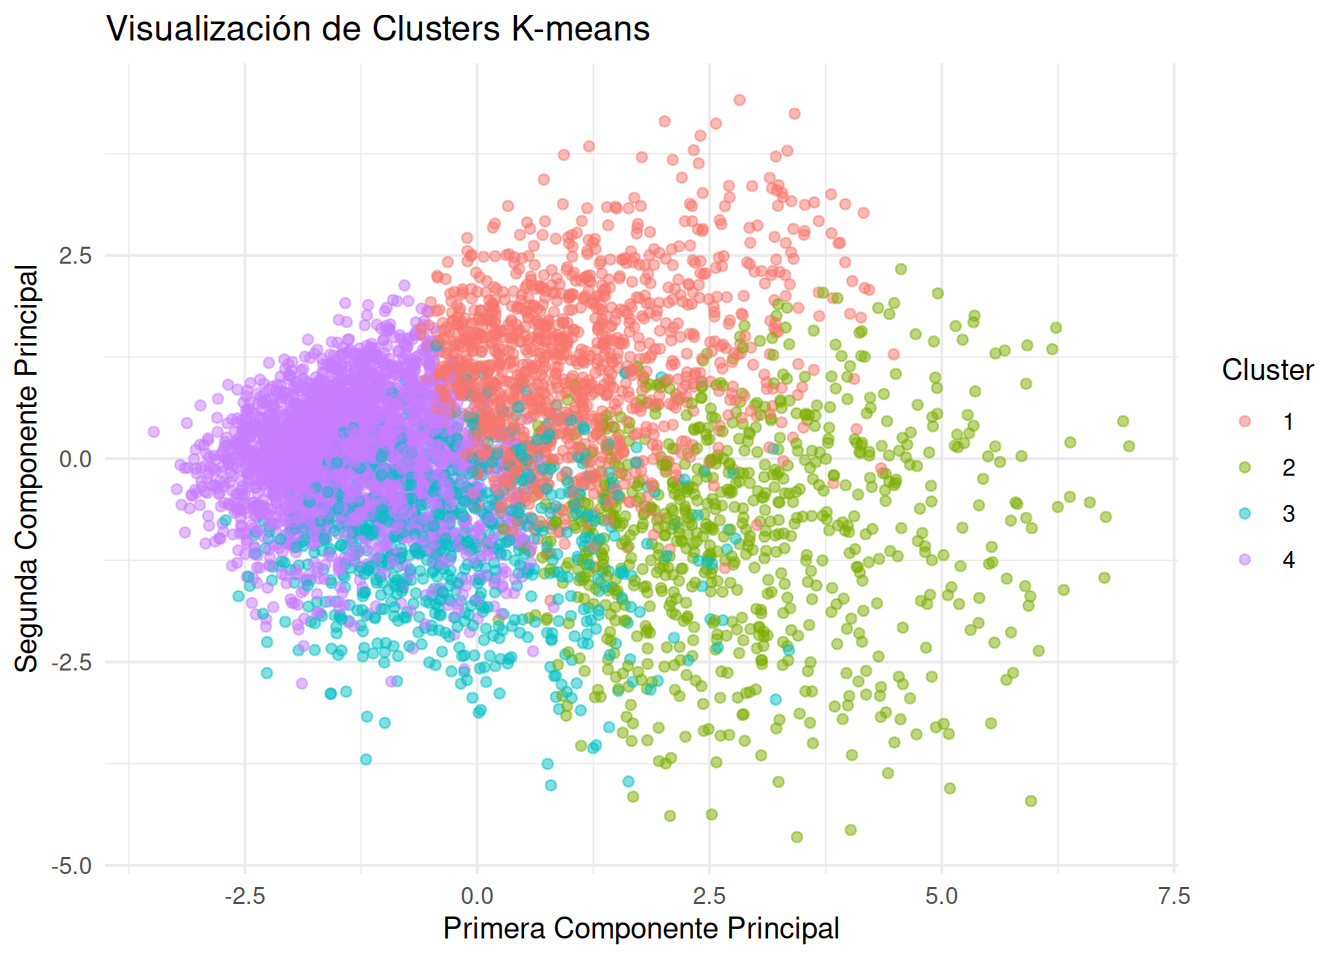
\includegraphics{Reporte_Entrega2_Proyecto1_files/figure-latex/unnamed-chunk-3-1.pdf}

\subsection{Análisis de componentes}\label{anuxe1lisis-de-componentes}

\subsubsection{3.1 ¿Qué variables categóricas serán
necesarias?}\label{quuxe9-variables-categuxf3ricas-seruxe1n-necesarias}

Primero se deben analizar cuáles variables serán importantes para el
análisis y cuáles pueden descartarse.

Las variables del dataset son: ID: es una variable cualitativa nominal,
pues sirve para identificar cada película

Popularity: es una variable cuantitativa medible continua pues es una
cantdad que puede medirse en base a ciertos criterios.

Budget: es una variable cuantitativa contable pues representa una
cantidad de dinero.

Revenue: es una variable cuantitativa contable ya que representa una
cantidad de dinero.

``Original title: es una variable cualitativa nominal ya que sirve para
identificar el nombre de cada película.''

Original language: es una variable cualitativa nominal ya que sirve para
indicar en que lenguaje se hizo la película originalmente.

Title: es una variable cualitativa nominal y sirve para indicar cuál es
el título en inglés de la película

Home page: es una variable cualitativa nominal y sirve para indicar si
la película tiene un sitio web.

Video: es una variable cualitativa nominal, pues sirve para idnciar si
la película tiene promocionales o no.

Director: es una variable cualitativa nominal la cua´l indica el nombre
del director de la película.

Runtime: es una variable cuantitativa continua medible, pues sirve para
indicar el tiempo de duración de la película el cuál puede ser
perfectamente medido con aparatos como un temporizador o cronómetro.

Genres: es una variable cualitativa nominal pues sirve para identificar
los géneros de la película.

Genres amount: es una variable cuantitativa discreta pues indica la
cantidad de géneros a los que pertence cada película.

Production company: es una variale cualitativa nominal la cual indica la
compañía que produjo la película.

Production company amount: es una variable cuantitativa discreta que
indica la cantidad de compañías involucradas en la producción de la
película.

Production company country: es una variable cualitativa nominal pues
sirve para indicar que países estuvieron involucrados en la producción
de la película.

Production countries amount: es una variable cuantitativa discreta la
cuál indica la cantidadde países involucrados en la producción de la
película.

Release date: es una variable cuantitativa nominal pues indica la fecha
de lanzamiento de la película. A pesar de ser numeral no es cuantitativa
pues no puede contarse.

Vote count: es una variable cuantitativa discreta pues indica la
cantidad de gente que reseñó la película.''

Vote average: es una variable

Actors: es una variable cualitativa nominal la cuál indica el nombre de
los actores involucrados en la película.

``Actors popularity: es una variable cuantitatva discreta la cuál sirve
panra indicar, en números decimales, que tan poular es un actor.''

Actor Character: es una variable cualitativa nominal pues sirve para
indicar el nombre del personaje que interpreta cada actor en la
película.

Actors amount: es una variable cuantitativa discreta pues indica la
cantidad de actores que están involucrados en la película.

Cast women amount: es una variable cuantitativa discreta la cuál indica
la cantidad de actrices que participaron en la película.

Cast men amount: es una variable cuantitativa discreta que indica la
canidad de actores que participaron el la película.

La variable ID y las variables que corresponden a los títulos de la
películas pueden descartarse, pues su único propósito es identificar
cada película. Otra variables descartables son las variables Actor
Character y Actors pues simplemente indican los nombres de los actores
involucrados en la película y los personajes a los que interpertan.

La variable video puede perecer descartable, sin embargo puede dar
información relevante para determinar el comportamiento de una película
pues podría ser que el hecho de tener videos ayude al rendimiento en
taquilla de una película o no. También podría ser útil para determinar
si el presupuesto de una película se ve afectado si tiene videos
promocionales.

La variable genres es de utilidad ya que puede ser de ayuda para
determinar si hay géneros de películas más famosos que otros o no, en el
análisis exploratorio se determióo que hay géneros de películas que han
obtenido mejores rendimientos en taquilla y que son más populares que
otros por lo que los géneros de una película pueden ser una pieza de
información relevante. Sin embargo la columna genres posee un formato
complicado el cuál aumentaría la dimensionalidad del dataset, por ende
se usuará la variable genres amount y se determinará si la diversidad de
géneros afecta el rendimiento de una película o si atrae a más cientes.

Si una película tiene o no un sitio web también puede ser relvante para
el análisis pues podría considerarse como parte de la promoción de la
película, por lo que esta variable puede ser de importancia para el
análisis.

La fecha de lanzamiento también es relevante pues en el análisis
exploratorio se demostró que hay épocas del año en donde las películas
obtienen mejores ingresos, por ende se requiere extraer el mes de
lanzamiento de cada película para el análisis.

La variable director es importante ya que hay directores más famosos que
otros sin embargo hay bastantes directores diferentes en el dataset, por
lo que asignarle un número a cada uno podría darnos un rango de números
bastante elevado. Por esa razón se convertirán ess valores a la cantidad
de directores involucrados y se analizara si la cantidad de directores
pesa en el desempeño de una película

El país de origen es importante, sin embargo hay películas, por esta
razón se usará la variable productionCountriesAmount y se determinará si
el hecho de que la película esté distribuida en más, o menos cantidad de
películas es importante o no.

El nombre de la distribuidora también es importante, sin embargo hay
muchas distribuidoras, por esa razón se usará la variable de production
amount para determinar si tener una o más productoras involucradas es
importante para la película.

El lenguaje original también puede ser un factor importante, por lo que
se convertirán a factores los valores de esta variable

\begin{Shaded}
\begin{Highlighting}[]
\CommentTok{\#Transformación de la data}

\NormalTok{movies\_pca }\OtherTok{\textless{}{-}}\NormalTok{movies}

\CommentTok{\#Convertimos las columnas relacionadas a los videos procionales}


\NormalTok{movies\_pca}\SpecialCharTok{$}\NormalTok{video[}\FunctionTok{is.na}\NormalTok{(movies\_pca}\SpecialCharTok{$}\NormalTok{video)] }\OtherTok{\textless{}{-}} \ConstantTok{FALSE}
\NormalTok{movies\_pca}\SpecialCharTok{$}\NormalTok{video}\OtherTok{\textless{}{-}} \FunctionTok{as.numeric}\NormalTok{(}\FunctionTok{factor}\NormalTok{(movies\_pca}\SpecialCharTok{$}\NormalTok{video)) }\CommentTok{\#2 true, 1 false}
\CommentTok{\#Trasnformamos los valores NA de la variable del website}
\NormalTok{movies\_pca}\SpecialCharTok{$}\NormalTok{homePage[}\SpecialCharTok{!}\FunctionTok{is.na}\NormalTok{(movies\_pca}\SpecialCharTok{$}\NormalTok{homePage)] }\OtherTok{\textless{}{-}} \ConstantTok{TRUE}
\NormalTok{movies\_pca}\SpecialCharTok{$}\NormalTok{homePage[}\FunctionTok{is.na}\NormalTok{(movies\_pca}\SpecialCharTok{$}\NormalTok{homePage)] }\OtherTok{\textless{}{-}} \ConstantTok{FALSE}
\NormalTok{movies\_pca}\SpecialCharTok{$}\NormalTok{homePage}\OtherTok{\textless{}{-}} \FunctionTok{as.numeric}\NormalTok{(}\FunctionTok{factor}\NormalTok{(movies\_pca}\SpecialCharTok{$}\NormalTok{homePage))  }\CommentTok{\#2 true, 1 false}

\NormalTok{movies\_pca }\OtherTok{\textless{}{-}} \FunctionTok{na.omit}\NormalTok{(movies\_pca)}

\CommentTok{\#Transformar el lenguage original}
\NormalTok{movies\_pca}\SpecialCharTok{$}\NormalTok{originalLanguage}\OtherTok{\textless{}{-}} \FunctionTok{as.numeric}\NormalTok{(}\FunctionTok{factor}\NormalTok{(movies\_pca}\SpecialCharTok{$}\NormalTok{originalLanguage))}


\CommentTok{\#Obtener los meses de lanzamiento de cada película}

\NormalTok{movies\_pca}\SpecialCharTok{$}\NormalTok{releaseDate }\OtherTok{\textless{}{-}} \FunctionTok{as.numeric}\NormalTok{(}\FunctionTok{format}\NormalTok{(}\FunctionTok{as.Date}\NormalTok{(movies\_pca}\SpecialCharTok{$}\NormalTok{releaseDate, }\AttributeTok{format=}\StringTok{"\%Y{-}\%m{-}\%d"}\NormalTok{), }\StringTok{"\%m"}\NormalTok{))}

\CommentTok{\#Cambiar los valores de la columna del director. }

\NormalTok{movies\_pca}\SpecialCharTok{$}\NormalTok{director }\OtherTok{\textless{}{-}} \FunctionTok{sapply}\NormalTok{(}\FunctionTok{gregexpr}\NormalTok{(}\StringTok{"}\SpecialCharTok{\textbackslash{}\textbackslash{}}\StringTok{|"}\NormalTok{, movies\_pca}\SpecialCharTok{$}\NormalTok{director), }\ControlFlowTok{function}\NormalTok{(x) }\FunctionTok{sum}\NormalTok{(x }\SpecialCharTok{\textgreater{}=} \DecValTok{0}\NormalTok{)) }\SpecialCharTok{+} \DecValTok{1}

\NormalTok{movies\_pca}\SpecialCharTok{$}\NormalTok{actorsPopularity }\OtherTok{\textless{}{-}} \FunctionTok{sapply}\NormalTok{(}\FunctionTok{strsplit}\NormalTok{(movies\_pca}\SpecialCharTok{$}\NormalTok{actorsPopularity, }\StringTok{"}\SpecialCharTok{\textbackslash{}\textbackslash{}}\StringTok{|"}\NormalTok{), }
                                  \ControlFlowTok{function}\NormalTok{(x) }\FunctionTok{mean}\NormalTok{(}\FunctionTok{as.numeric}\NormalTok{(x), }\AttributeTok{na.rm =} \ConstantTok{TRUE}\NormalTok{))}

\NormalTok{movies\_pca}\SpecialCharTok{$}\NormalTok{castWomenAmount }\OtherTok{\textless{}{-}} \FunctionTok{as.integer}\NormalTok{(movies\_pca}\SpecialCharTok{$}\NormalTok{castWomenAmount)}
\NormalTok{movies\_pca}\SpecialCharTok{$}\NormalTok{castMenAmount }\OtherTok{\textless{}{-}} \FunctionTok{as.integer}\NormalTok{(movies\_pca}\SpecialCharTok{$}\NormalTok{castMenAmount)}
\end{Highlighting}
\end{Shaded}

\subsubsection{3.2 ¿Es conveniente hacer
PCA?}\label{es-conveniente-hacer-pca}

\begin{Shaded}
\begin{Highlighting}[]
\FunctionTok{library}\NormalTok{(psych)}
\end{Highlighting}
\end{Shaded}

\begin{verbatim}
## 
## Attaching package: 'psych'
\end{verbatim}

\begin{verbatim}
## The following objects are masked from 'package:ggplot2':
## 
##     %+%, alpha
\end{verbatim}

\begin{Shaded}
\begin{Highlighting}[]
\FunctionTok{library}\NormalTok{(FactoMineR)}
\FunctionTok{library}\NormalTok{(factoextra)}
\FunctionTok{library}\NormalTok{(corrplot)}
\end{Highlighting}
\end{Shaded}

\begin{verbatim}
## corrplot 0.95 loaded
\end{verbatim}

\begin{Shaded}
\begin{Highlighting}[]
\NormalTok{movies\_final }\OtherTok{\textless{}{-}}\NormalTok{ movies\_pca[, }\FunctionTok{c}\NormalTok{(}\StringTok{"budget"}\NormalTok{, }\StringTok{"homePage"}\NormalTok{, }\StringTok{"revenue"}\NormalTok{, }\StringTok{"runtime"}\NormalTok{, }\StringTok{"video"}\NormalTok{, }\StringTok{"director"}\NormalTok{, }\StringTok{"actorsPopularity"}\NormalTok{, }\StringTok{"originalLanguage"}\NormalTok{, }\StringTok{"popularity"}\NormalTok{, }\StringTok{"releaseDate"}\NormalTok{, }\StringTok{"voteAvg"}\NormalTok{, }\StringTok{"voteCount"}\NormalTok{, }\StringTok{"genresAmount"}\NormalTok{, }\StringTok{"productionCoAmount"}\NormalTok{, }\StringTok{"productionCountriesAmount"}\NormalTok{, }\StringTok{"actorsAmount"}\NormalTok{, }\StringTok{"castWomenAmount"}\NormalTok{, }\StringTok{"castMenAmount"}\NormalTok{ )]}


\NormalTok{rcor }\OtherTok{\textless{}{-}} \FunctionTok{cor}\NormalTok{(movies\_final, }\AttributeTok{use =} \StringTok{"pairwise.complete.obs"}\NormalTok{)}
\FunctionTok{det}\NormalTok{(rcor)}
\end{Highlighting}
\end{Shaded}

\begin{verbatim}
## [1] 0.05361342
\end{verbatim}

El valor del determinate de la matriz es de 0.0536134, es más cercano a
0 que a 1, por lo que se puede decir que las variables si están
relacionadas

\paragraph{KMO}\label{kmo}

\begin{Shaded}
\begin{Highlighting}[]
\FunctionTok{KMO}\NormalTok{(}\FunctionTok{as.matrix}\NormalTok{(movies\_final))}
\end{Highlighting}
\end{Shaded}

\begin{verbatim}
## Kaiser-Meyer-Olkin factor adequacy
## Call: KMO(r = as.matrix(movies_final))
## Overall MSA =  0.64
## MSA for each item = 
##                    budget                  homePage                   revenue 
##                      0.75                      0.85                      0.68 
##                   runtime                     video                  director 
##                      0.69                      0.44                      0.63 
##          actorsPopularity          originalLanguage                popularity 
##                      0.63                      0.49                      0.79 
##               releaseDate                   voteAvg                 voteCount 
##                      0.52                      0.53                      0.74 
##              genresAmount        productionCoAmount productionCountriesAmount 
##                      0.62                      0.55                      0.46 
##              actorsAmount           castWomenAmount             castMenAmount 
##                      0.34                      0.37                      0.45
\end{verbatim}

Se obtuvo que el MSA es de 0.64, por lo que la adecuación muestral para
el análisis factorial es aceptable.

\paragraph{Prueba esfericidad de
Bartlett.}\label{prueba-esfericidad-de-bartlett.}

Por último se hará este prueba para verificar completamente si se puede
hacer un análisis de componentes sobre el dataset

\begin{Shaded}
\begin{Highlighting}[]
\FunctionTok{cortest.bartlett}\NormalTok{(rcor)}
\end{Highlighting}
\end{Shaded}

\begin{verbatim}
## $chisq
## [1] 269.6756
## 
## $p.value
## [1] 1.799032e-08
## 
## $df
## [1] 153
\end{verbatim}

El p value es de 1.799032e-08, por lo que este test también sugiere que
es adecuado hacer un análisis de componentes.

\subsection{Interpretacion de los
resultados}\label{interpretacion-de-los-resultados}

\begin{Shaded}
\begin{Highlighting}[]
\NormalTok{movies\_clean}\SpecialCharTok{$}\NormalTok{cluster }\OtherTok{\textless{}{-}} \FunctionTok{as.factor}\NormalTok{(kmeans\_result}\SpecialCharTok{$}\NormalTok{cluster)}

\CommentTok{\# Estadísticas descriptivas por cluster}
\NormalTok{cluster\_stats }\OtherTok{\textless{}{-}}\NormalTok{ movies\_clean }\SpecialCharTok{\%\textgreater{}\%}
  \FunctionTok{group\_by}\NormalTok{(cluster) }\SpecialCharTok{\%\textgreater{}\%}
  \FunctionTok{summarise}\NormalTok{(}
    \AttributeTok{n =} \FunctionTok{n}\NormalTok{(),}
    \CommentTok{\# Medidas de tendencia central}
    \AttributeTok{avg\_budget =} \FunctionTok{mean}\NormalTok{(budget, }\AttributeTok{na.rm =} \ConstantTok{TRUE}\NormalTok{),}
    \AttributeTok{avg\_revenue =} \FunctionTok{mean}\NormalTok{(revenue, }\AttributeTok{na.rm =} \ConstantTok{TRUE}\NormalTok{),}
    \AttributeTok{avg\_runtime =} \FunctionTok{mean}\NormalTok{(runtime, }\AttributeTok{na.rm =} \ConstantTok{TRUE}\NormalTok{),}
    \AttributeTok{avg\_popularity =} \FunctionTok{mean}\NormalTok{(popularity, }\AttributeTok{na.rm =} \ConstantTok{TRUE}\NormalTok{),}
    \AttributeTok{avg\_vote =} \FunctionTok{mean}\NormalTok{(voteAvg, }\AttributeTok{na.rm =} \ConstantTok{TRUE}\NormalTok{),}
    \AttributeTok{avg\_vote\_count =} \FunctionTok{mean}\NormalTok{(voteCount, }\AttributeTok{na.rm =} \ConstantTok{TRUE}\NormalTok{),}
    \AttributeTok{avg\_actors =} \FunctionTok{mean}\NormalTok{(actorsAmount, }\AttributeTok{na.rm =} \ConstantTok{TRUE}\NormalTok{),}
    \AttributeTok{avg\_women =} \FunctionTok{mean}\NormalTok{(castWomenAmount, }\AttributeTok{na.rm =} \ConstantTok{TRUE}\NormalTok{),}
    \AttributeTok{avg\_men =} \FunctionTok{mean}\NormalTok{(castMenAmount, }\AttributeTok{na.rm =} \ConstantTok{TRUE}\NormalTok{),}
    \CommentTok{\# Medidas de dispersión}
    \AttributeTok{sd\_budget =} \FunctionTok{sd}\NormalTok{(budget, }\AttributeTok{na.rm =} \ConstantTok{TRUE}\NormalTok{),}
    \AttributeTok{sd\_revenue =} \FunctionTok{sd}\NormalTok{(revenue, }\AttributeTok{na.rm =} \ConstantTok{TRUE}\NormalTok{),}
    \CommentTok{\# Métricas derivadas}
    \AttributeTok{roi =}\NormalTok{ (}\FunctionTok{mean}\NormalTok{(revenue, }\AttributeTok{na.rm =} \ConstantTok{TRUE}\NormalTok{) }\SpecialCharTok{{-}} \FunctionTok{mean}\NormalTok{(budget, }\AttributeTok{na.rm =} \ConstantTok{TRUE}\NormalTok{)) }\SpecialCharTok{/} \FunctionTok{mean}\NormalTok{(budget, }\AttributeTok{na.rm =} \ConstantTok{TRUE}\NormalTok{)}
\NormalTok{  )}

\FunctionTok{print}\NormalTok{(}\StringTok{"Análisis de Clusters:"}\NormalTok{)}
\end{Highlighting}
\end{Shaded}

\begin{verbatim}
## [1] "Análisis de Clusters:"
\end{verbatim}

\begin{Shaded}
\begin{Highlighting}[]
\FunctionTok{print}\NormalTok{(cluster\_stats)}
\end{Highlighting}
\end{Shaded}

\begin{verbatim}
## # A tibble: 4 x 14
##   cluster     n avg_budget avg_revenue avg_runtime avg_popularity avg_vote
##   <fct>   <int>      <dbl>       <dbl>       <dbl>          <dbl>    <dbl>
## 1 1        1315   4717988.    7409286.       106.            19.4     6.56
## 2 2         796  25109075.   54828551.       106.            26.5     6.43
## 3 3         873   4673659.    4914797.       101.            20.5     6.33
## 4 4        2513   1666754.    2610763.        93.9           23.9     6.29
## # i 7 more variables: avg_vote_count <dbl>, avg_actors <dbl>, avg_women <dbl>,
## #   avg_men <dbl>, sd_budget <dbl>, sd_revenue <dbl>, roi <dbl>
\end{verbatim}

\begin{Shaded}
\begin{Highlighting}[]
\CommentTok{\# Presupuesto vs Ingresos}
\FunctionTok{ggplot}\NormalTok{(movies\_clean, }\FunctionTok{aes}\NormalTok{(}\AttributeTok{x =}\NormalTok{ budget, }\AttributeTok{y =}\NormalTok{ revenue, }\AttributeTok{color =}\NormalTok{ cluster)) }\SpecialCharTok{+}
  \FunctionTok{geom\_point}\NormalTok{(}\AttributeTok{alpha =} \FloatTok{0.5}\NormalTok{) }\SpecialCharTok{+}
  \FunctionTok{theme\_minimal}\NormalTok{() }\SpecialCharTok{+}
  \FunctionTok{labs}\NormalTok{(}\AttributeTok{title =} \StringTok{"Presupuesto vs Ingresos por Cluster"}\NormalTok{,}
       \AttributeTok{x =} \StringTok{"Presupuesto"}\NormalTok{,}
       \AttributeTok{y =} \StringTok{"Ingresos"}\NormalTok{)}
\end{Highlighting}
\end{Shaded}

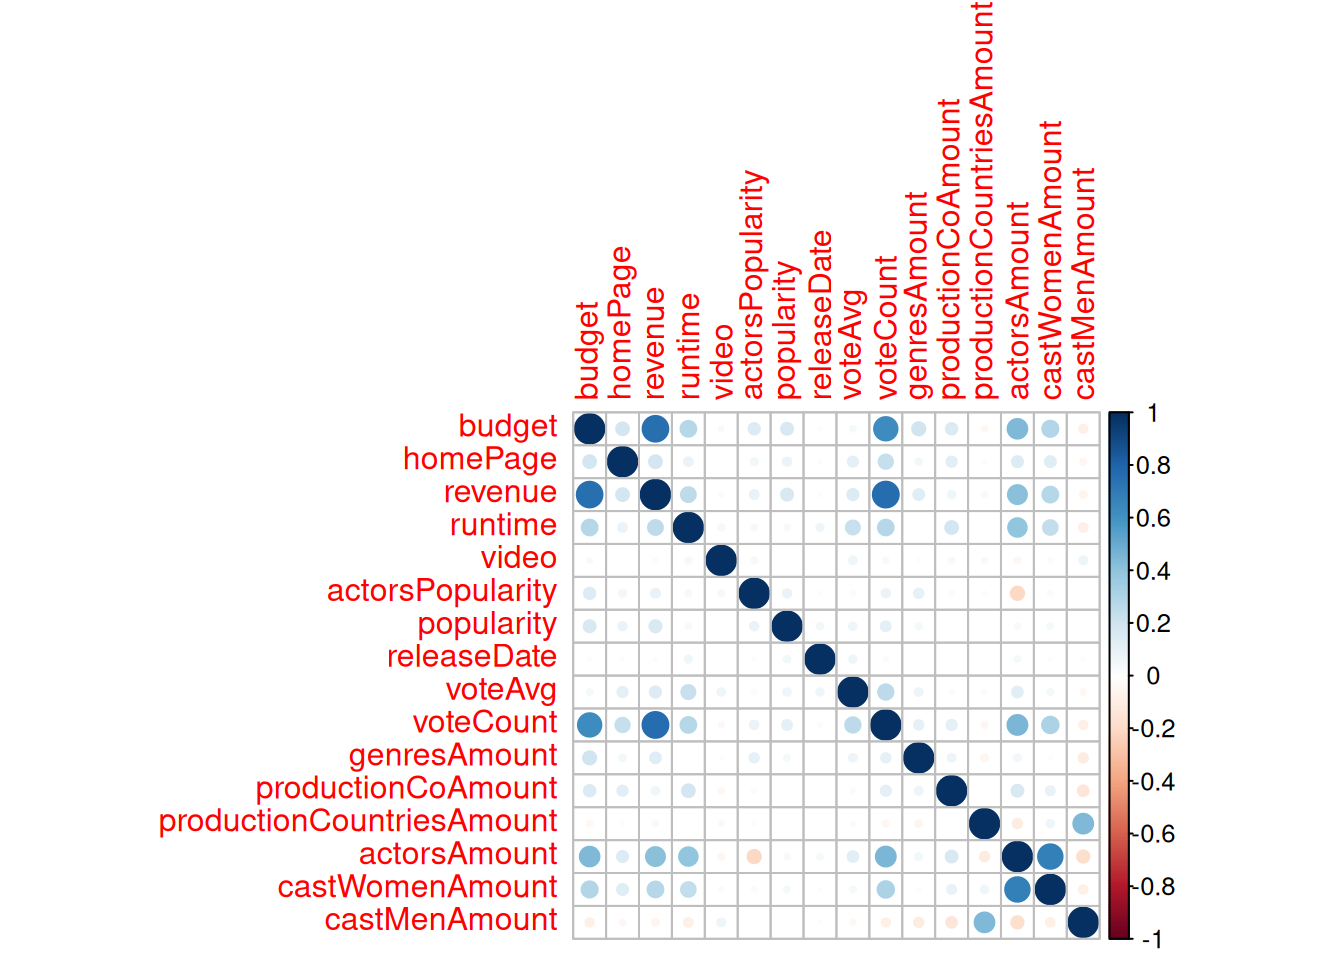
\includegraphics{Reporte_Entrega2_Proyecto1_files/figure-latex/unnamed-chunk-8-1.pdf}

\begin{Shaded}
\begin{Highlighting}[]
\CommentTok{\# Popularidad vs Calificación promedio}
\FunctionTok{ggplot}\NormalTok{(movies\_clean, }\FunctionTok{aes}\NormalTok{(}\AttributeTok{x =}\NormalTok{ popularity, }\AttributeTok{y =}\NormalTok{ voteAvg, }\AttributeTok{color =}\NormalTok{ cluster)) }\SpecialCharTok{+}
  \FunctionTok{geom\_point}\NormalTok{(}\AttributeTok{alpha =} \FloatTok{0.5}\NormalTok{) }\SpecialCharTok{+}
  \FunctionTok{theme\_minimal}\NormalTok{() }\SpecialCharTok{+}
  \FunctionTok{labs}\NormalTok{(}\AttributeTok{title =} \StringTok{"Popularidad vs Calificación por Cluster"}\NormalTok{,}
       \AttributeTok{x =} \StringTok{"Popularidad"}\NormalTok{,}
       \AttributeTok{y =} \StringTok{"Calificación Promedio"}\NormalTok{)}
\end{Highlighting}
\end{Shaded}

\includegraphics{Reporte_Entrega2_Proyecto1_files/figure-latex/unnamed-chunk-8-2.pdf}

\#\#\#Interpretación de los Grupos y Hallazgos Distribución de los
Clusters (K-means)

La distribución de clusters ordenadas de mayor a menor, me dio lo
siguiente:

Cluster 4: 2,513 películas (45.6\%), representando la mayoría de las
producciones con características promedio. Cluster 1: 1,315 películas
(24.0\%), con características que se desvían moderadamente del estándar.
Cluster 3: 873 películas (15.9\%), probablemente películas
independientes o de menor inversión. Cluster 2: 796 películas (14.5\%),
caracterizadas por mayor presupuesto e impacto en la industria.

\#\#\#\#Calidad del Agrupamiento

El coeficiente de silueta obtenido fue de 0.145 para K-means y 0.105
para clustering jerárquico. Aunque ambos valores son relativamente
bajos, K-means mostró una mejor separación de grupos, lo que justifica
su uso en la interpretación. Análisis Visual mediante PCA

\begin{itemize}
\tightlist
\item
  Cluster 4 se encuentra en una posición central y densa, lo que sugiere
  que representa la categoría más común de películas.
\item
  Cluster 2 se extiende hacia la derecha, indicando valores elevados en
  ciertas métricas.
\item
  Cluster 3 se agrupa en la parte inferior del espacio PCA, reflejando
  un presupuesto menor.
\item
  Cluster 1 presenta una distribución más dispersa, lo que sugiere una
  mayor variabilidad en sus características.
\end{itemize}

\paragraph{Relevancia para la
Industria}\label{relevancia-para-la-industria}

Los resultados reflejan una estructura de mercado donde:

\begin{itemize}
\tightlist
\item
  La mayoría de las películas siguen un patrón estándar (Cluster 4).
\item
  Las superproducciones representan un segmento más reducido pero
  influyente (Cluster 2).
\item
  Existe un mercado intermedio de películas con impacto moderado
  (Cluster 1).
\item
  Se mantiene un sector significativo de producciones de menor
  presupuesto (Cluster 3).
\end{itemize}

\end{document}
